\section{Assembly of Algorithms and Information Flow In Concrete Implemention}

In section ~\ref{ch:scenario}, an overview was given of how algorithms work together in the system. In-depth implementation-specific details of this assembly and information flow will now be given.

\subsection{Library Visualization}

\begin{itemize}
	\item Extraction of music metadata on the device \\\\
			\textbf{Input:} Access cursor to a data store containing the device's music library metadata.  \\
			\textbf{Algorithm:} Iterates through all artists and tracks in the device's music library.
			If an entity has not yet been registered in the app's database, parts of its metadata are 
			compiled and put into the database. \\
			\textbf{Output:} Local music metadata stored in the app's database.\\
			
	\item Matching of the device's music metadata with metadata from web sources \\\\
			\textbf{Input:} Local music metadata stored in the app's database.  \\
			\textbf{Algorithm:} Iterates through all local music metadata previously retrieved, and calls
			Last.fm's RESTful API to find matching entities - picking the first match as best match. These pieces
			of remote metadata are then stored in the app's database. \\
			\textbf{Output:} Remote music metadata stored in the app's database. \\
			
	\item Querying of Artist Similarity data from web sources \\\\
			\textbf{Input:} Local music metadata and matched metadata from remote web sources stored in the app's database. \\
			\textbf{Algorithm:} Iterates through all local and remote music metadata previously retrieved, and calls
			Last.fm's RESTful API to get the 100 most similar artists for each. \\
			\textbf{Output:} Artist similarity relations stored in the app's database. \\
			
	\item Completion of Artist Similarity data \\\\
			\textbf{Input:} Artist similarity relations stored in the app's database. \\
			\textbf{Algorithm:} Iterates through the previously retrieved artist similarity relations, and
			adds approximations for similarity relations which have not been found in the web API's results.
			These approximations are calculated as described in section ~\ref{ch:computation}. \\
			\textbf{Output:} Complete artist similarity relations stored in the app's database. \\
			
	\item Laying out artists in 2D space with a Multi Dimensional Scaling (MDS) algorithm \\\\
			\textbf{Input:} Complete artist similarity relations stored in the app's database.   \\
			\textbf{Algorithm:} Applies a multistep (see sub-steps) algorithm which uses previously
			retrieved similarity data to position nodes resembling artists without overlappings.  \\
			\textbf{Output:} Graph strucure of nodes resembling artists, laid out such that their position 
			indicates their similarity to each other. \\
			
		\subitem Building up of a distance matrix between artists \\\\
				\textbf{Input:} Complete artist similarity relations stored in the app's database. \\
				\textbf{Algorithm:} Iterates through all artist similarity relations, calculates a
				distance value (\emph{d = Similarity * -1 + 1}, d $\in$ [0, 1] ), and writes it into
				a matrix data structure where both dimensions' labels consist of all existing artists. \\
				\textbf{Output:} Distance matrix of artists, based on their inverted similarities. \\
				
		\subitem Generation of a subset of artists and laying them out according to spring model forces	\\\\
				\textbf{Input:} Distance matrix of artists, based on their inverted similarities. \\
				\textbf{Algorithm:} Picks a random sample of artists, assigns random positions to them,
				and applies a multi-dimensional scaling algorithm on them (see subsection 
				~\ref{subch:implementation-mds} later in this section). \\
				\textbf{Output:} Graph structure of nodes resembling artists (correctly positioned subset) \\
				
		\subitem Addition of the remaining artists, positioning them around the initial subset \\\\
				\textbf{Input:} Graph structure of nodes resembling artists (correctly positioned subset) \\
				\textbf{Algorithm:} Iterates through the remaining artist nodes and positions each on a position
				next to its most similar artist (estimating which quadrant will be the best). \\
				\textbf{Output:} Graph structure of nodes resembling artists, many of them suboptimally positioned \\
				
		\subitem Application of spring model forces on all nodes for a few iterations \\\\
				\textbf{Input:} Graph structure of nodes resembling artists, many of them suboptimally positioned \\
				\textbf{Algorithm:} Applies the aforementioned multi-dimensional algorithm on the whole graph of
				all artist nodes, thus reducing system stress (finding a better position for each artist).  \\
				\textbf{Output:} Graph strucure of nodes resembling artists, laid out such that their position 
				indicates their similarity to each other.\\
				
	\item Removal of overlapping of artists' depictions in 2D space	\\\\
				\textbf{Input:} Graph strucure of nodes resembling artists, laid out such that their position 
				indicates their similarity to each other. \\
				\textbf{Algorithm:} Empties out the graph, and re-adds the artist nodes back into it, one by one,
				while optionally moving nodes when they are added such that they do not overlap any other nodes. This
				movement is determined by the vector of both node's center coordinates and their amount
				of overlapping. For more details about this algorithm, see 
				~\ref{subch:implementation-overlapping} later in this section. \\
				\textbf{Output:} Graph strucure of nodes resembling artists, laid out such that they don't 
				overlap each other and their position indicates their similarity to each other. \\
				
	\item Display of the laid out artists in OpenGL	\\\\
				\textbf{Input:} Graph strucure of nodes resembling artists, laid out such that they don't 
				overlap each other and their position indicates their similarity to each other. \\
				\textbf{Algorithm:} Displays the graph on an OpenGL canvas (3D), by using the artists' images (in form
				of textures) and their names (rendered to textures). Sets the viewport and transformation
				matrices such that a 2D view is simulated, displaying artist nodes as viewed from above. \\
				\textbf{Output:} OpenGL view object and auxiliary system objects \\
				
	\item Continuous reaction to user actions (zooming, panning, tapping) \\\\
				\textbf{Input:} OpenGL view object and auxiliary system objects. \\
				\textbf{Algorithm:} Continuously reacts to user interface inputs, by moving the OpenGL canvas'
				pseudo-camera (i.e., manipulating the model transformation matrix) for zooming and panning.
				Marks an artist node as selected when the user taps onto it, and displays a context menu. \\
				\textbf{Output:} -
\end{itemize}

\subsection{Artist Discovery}

\begin{itemize}
	\item Querying of the artists most similar to "'subject"' from web sources \\\\
				\textbf{Input:} "'Subject"' artist the user has selected for discovery. \\
				\textbf{Algorithm:} Queries Last.fm for the artists most similar to "'subject"', and returns
				an excerpt of those. \\
				\textbf{Output:} Excerpt of artists most similar to "'subject"'. \\
	\item Integration of the retrieved artists around "'subject"' in 2D space, at randomized but similar positions \\\\
				\textbf{Input:} Excerpt of artists most similar to "'subject"'. \\
				\textbf{Algorithm:} Applies a force-based layout algorithm on the collection of "'subject"' and
				its similar artists, such that the similar artists are arranged in a star around "'subject"'. \\
				\textbf{Output:} Graph strucure of nodes resembling artists, laid out such that similar
				artists encircle "'subject"'. \\
	\item Continuous re-arrangement of the retrieved artists based on a force-based layout algorithm (also reacting to newly added similar artists) \\\\
				\textbf{Input:} Graph strucure of nodes resembling artists, laid out such that similar
				artists encircle "'subject"'. \\
				\textbf{Algorithm:} As the user selects more artist nodes as "'subject"' and load
				its similar artists, this algorithm is then restarted, but the previous subjects and their
				similar artists are kept, and their positions adapted as needed - i.e., force-based layout
				calculation does not stop for those. \\
				\textbf{Output:} - \\
\end{itemize}

\section{Algorithms with Screenshots}

\begin{figure}[H]
  \centering
    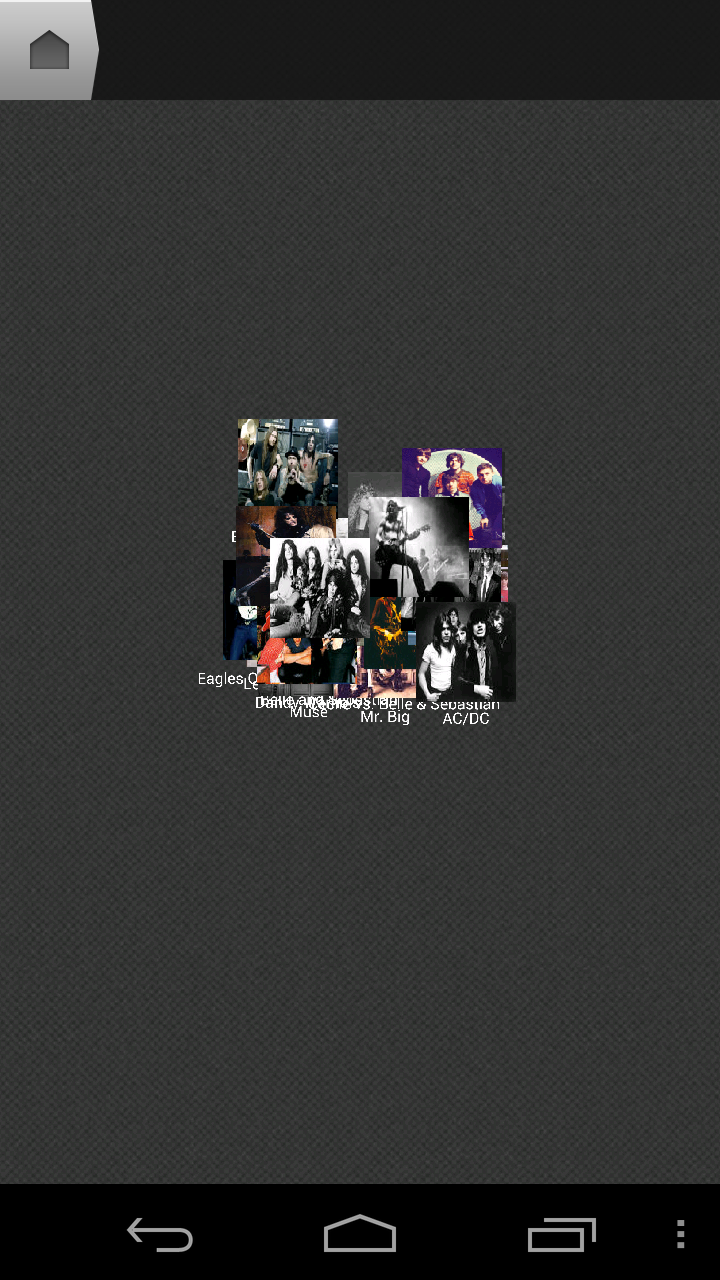
\includegraphics[width=0.4\textwidth]{figures/screen_mds_1_initial}
  \caption{The initial graph state before MDS calculation}
\end{figure}

\begin{figure}[H]
  \centering
    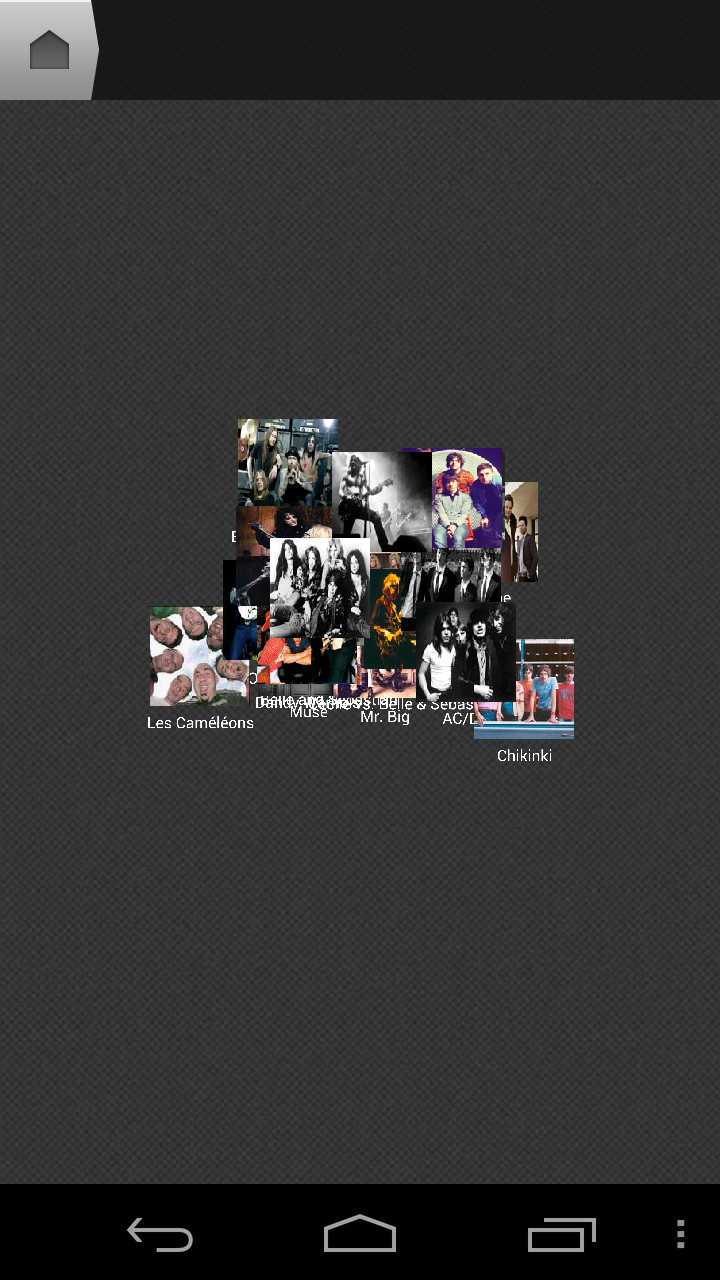
\includegraphics[width=0.4\textwidth]{figures/screen_mds_2_after_5_subset_iterations}
  \caption{Graph state after 5 iterations of the initial subset}
\end{figure}

\begin{figure}[H]
  \centering
    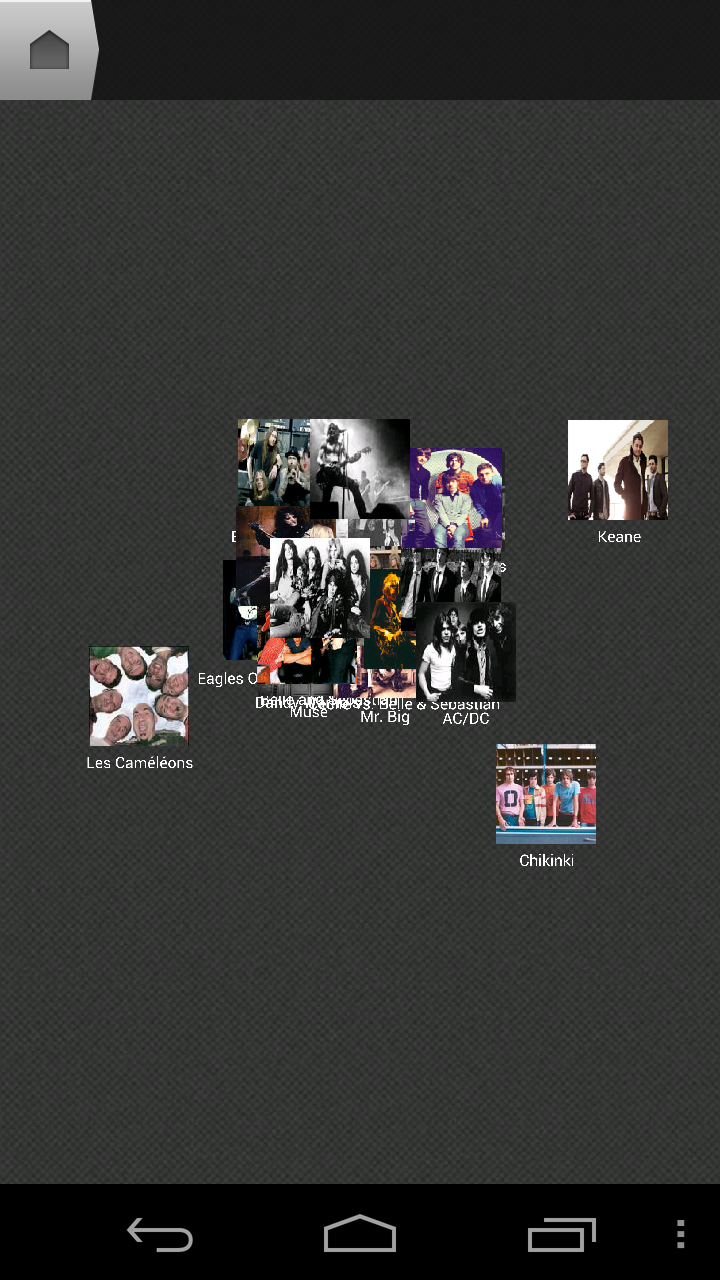
\includegraphics[width=0.4\textwidth]{figures/screen_mds_3_after_20_subset_iterations}
  \caption{Graph state after 20 spring force iterations of the initial subset}
\end{figure}

\begin{figure}[H]
  \centering
    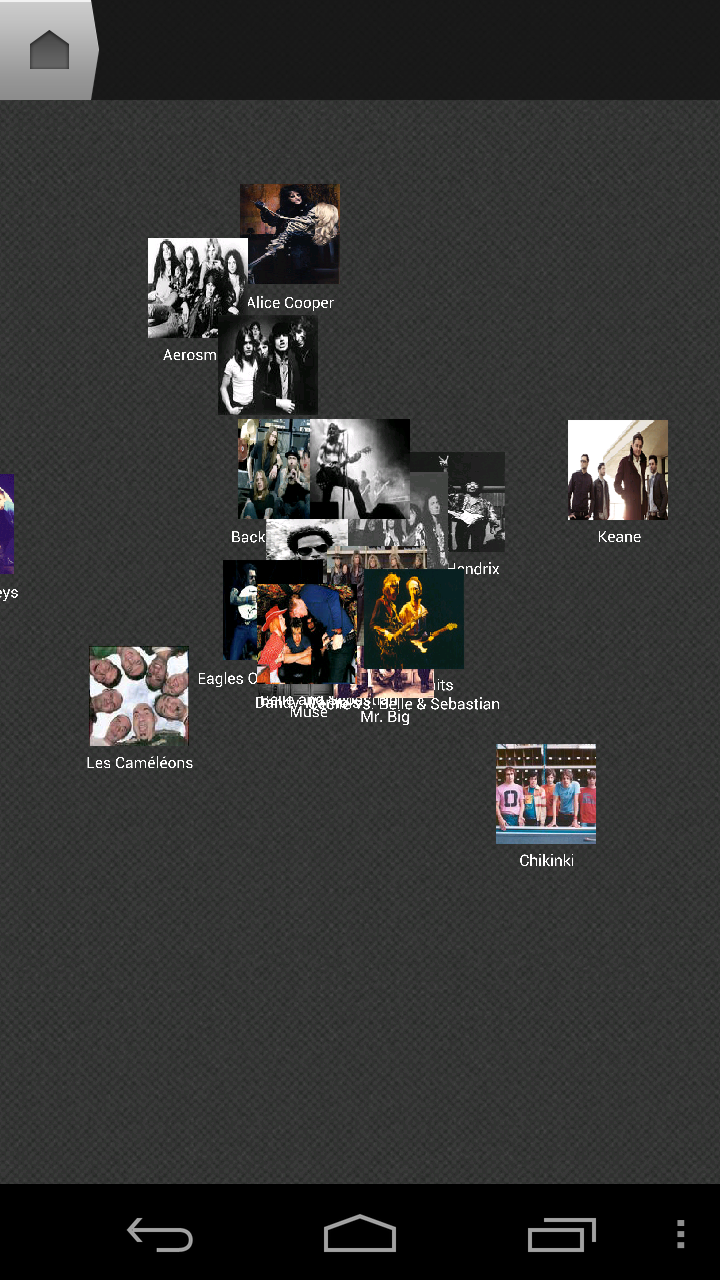
\includegraphics[width=0.4\textwidth]{figures/screen_mds_4_after_5_restnode_additions}
  \caption{Graph state after 5 placements of nodes outside the initial subset}
\end{figure}

\begin{figure}[H]
  \centering
    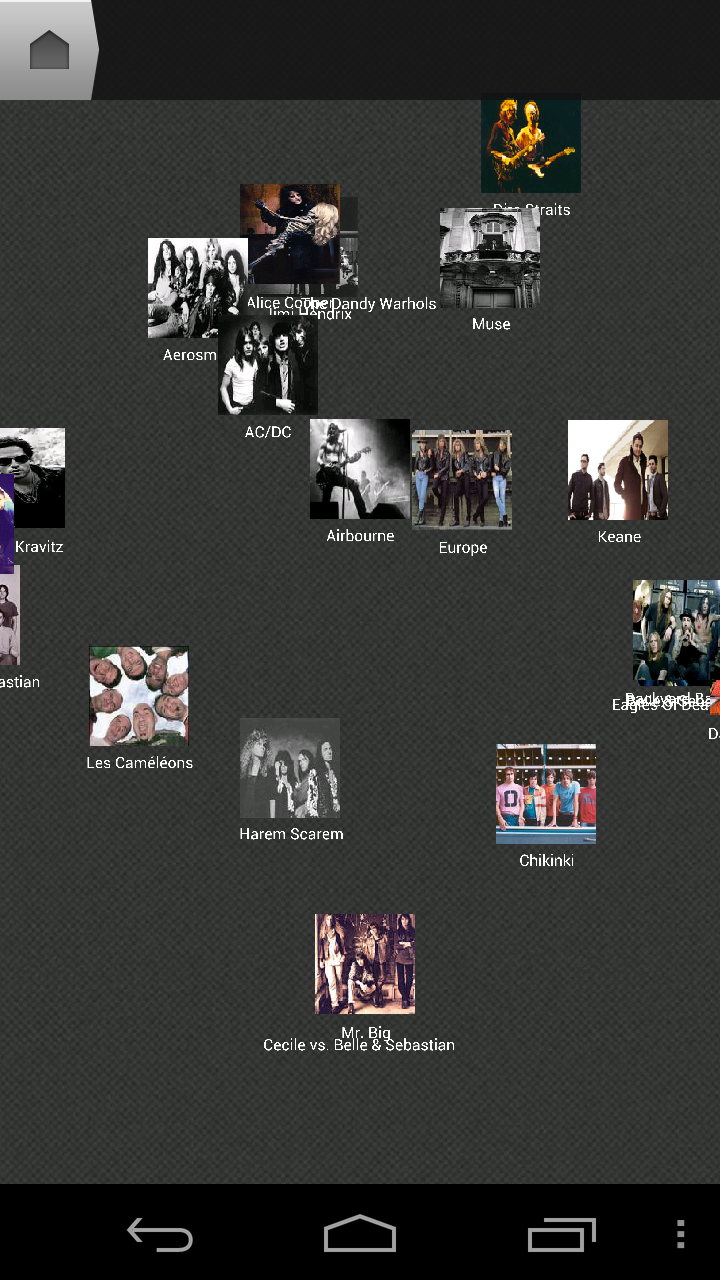
\includegraphics[width=0.4\textwidth]{figures/screen_mds_5_after_all_restnode_additions}
  \caption{Graph state after placements of all nodes outside the initial subset}
\end{figure}

\begin{figure}[H]
  \centering
    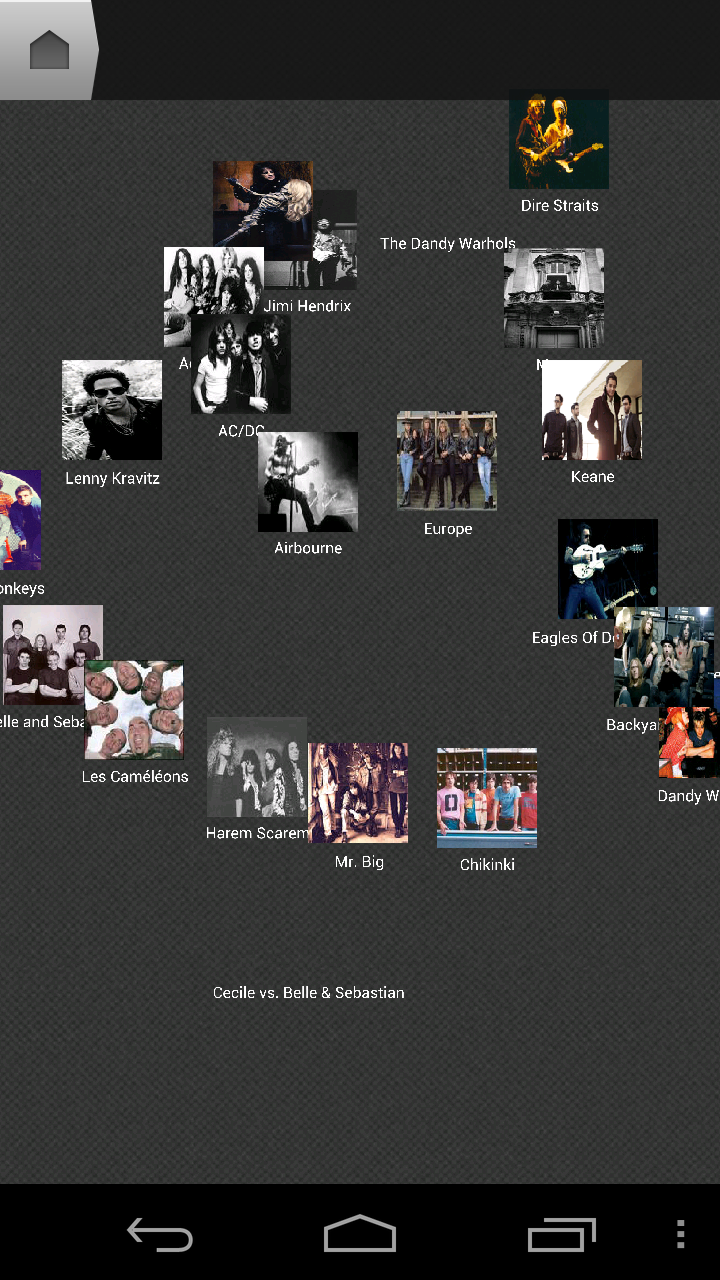
\includegraphics[width=0.4\textwidth]{figures/screen_mds_6_after_5_cleanup_iterations}
  \caption{Graph state after 5 spring force iterations of all nodes}
\end{figure}

\begin{figure}[H]
  \centering
    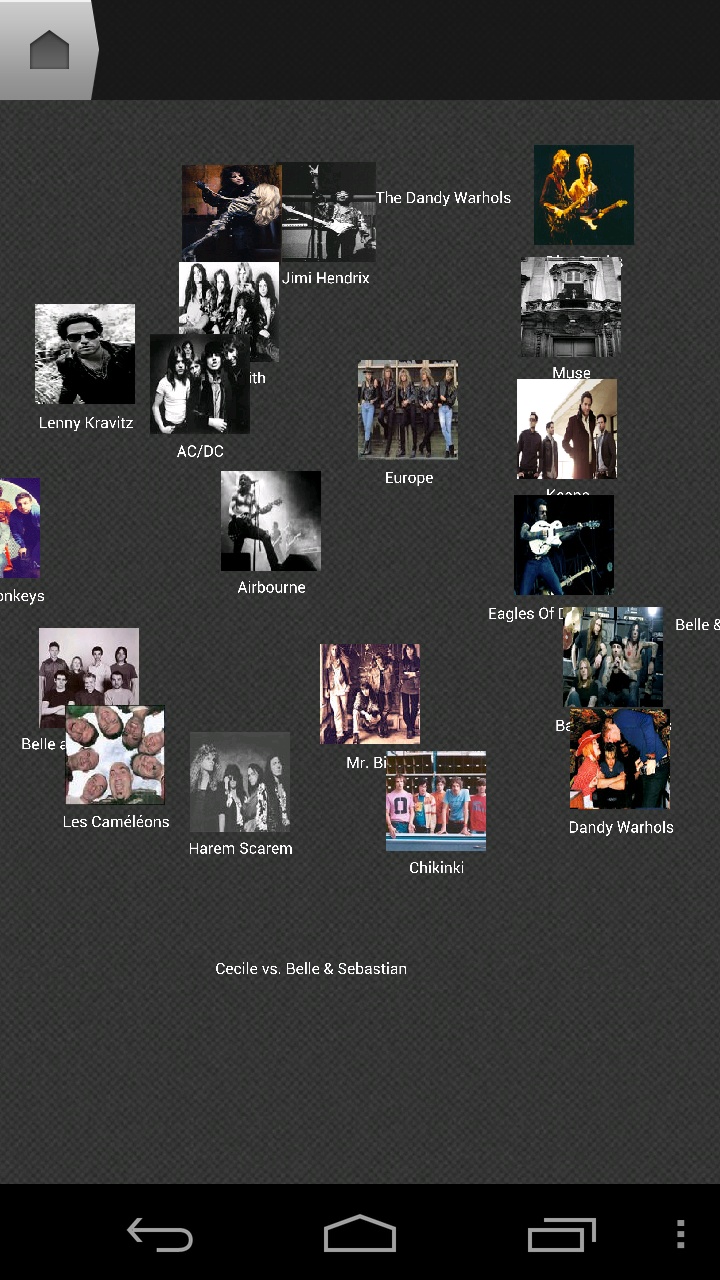
\includegraphics[width=0.4\textwidth]{figures/screen_mds_7_after_10_cleanup_iterations}
  \caption{Graph state after 10 spring force iterations of all nodes}
\end{figure}

\begin{figure}[H]
  \centering
    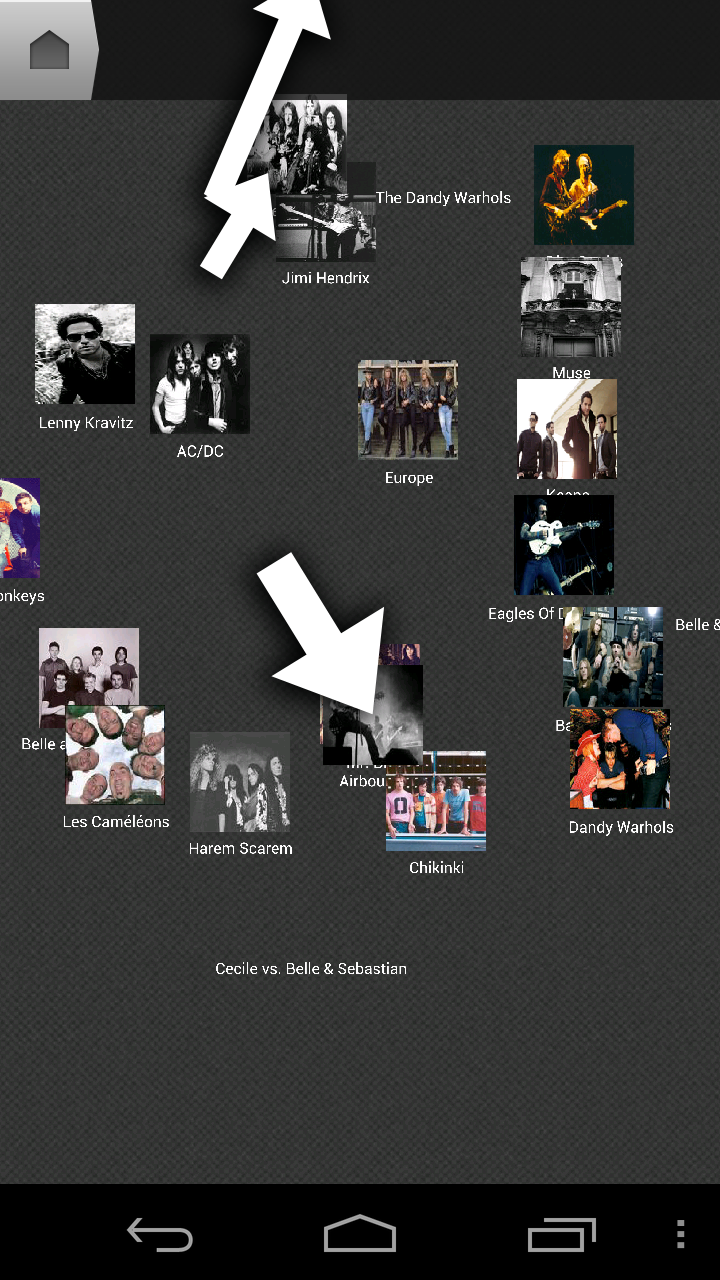
\includegraphics[width=0.4\textwidth]{figures/screen_mds_8_after_5_uncollided_nodes}
  \caption{Graph state after removal of node overlappings from 5 nodes}
\end{figure}

\begin{figure}[H]
  \centering
    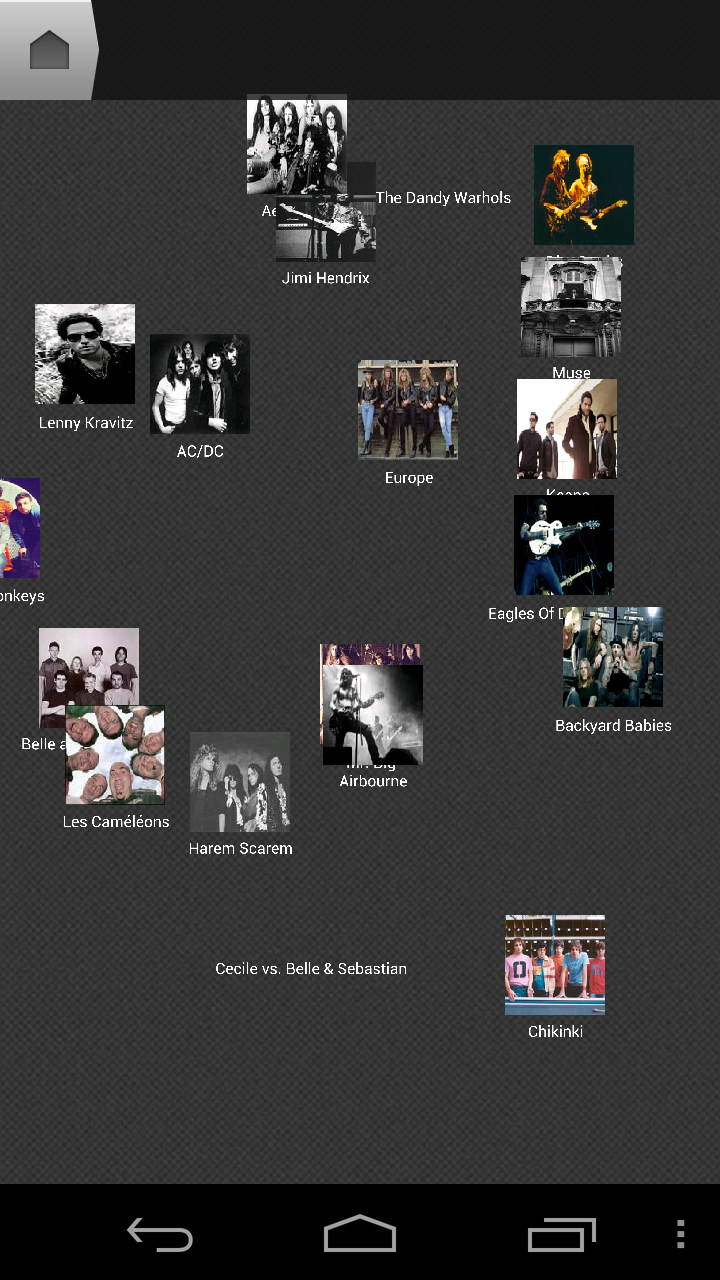
\includegraphics[width=0.4\textwidth]{figures/screen_mds_9_after_half_uncollided_nodes}
  \caption{Graph state after removal of node overlappings from half of all nodes}
\end{figure}

\begin{figure}[H]
  \centering
    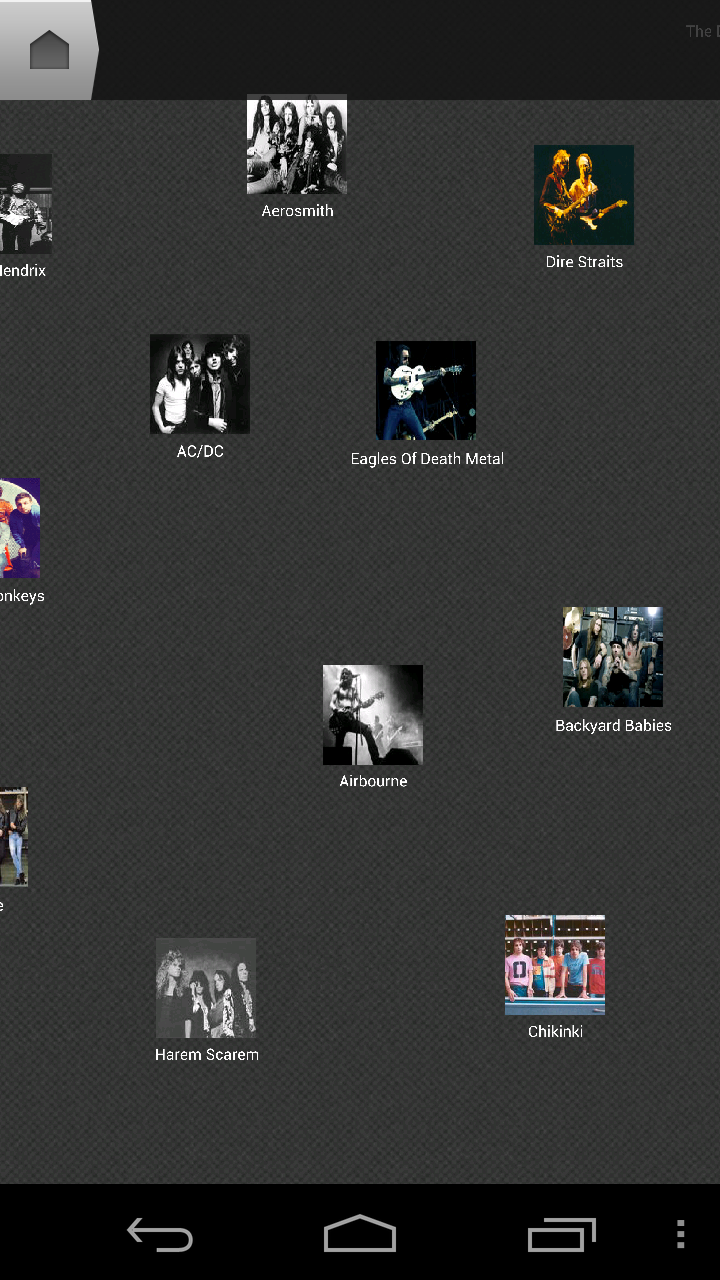
\includegraphics[width=0.4\textwidth]{figures/screen_mds_10_after_all_uncollided_nodes}
  \caption{Graph state after removal of node overlappings from all nodes}
\end{figure}

\begin{figure}[H]
  \centering
    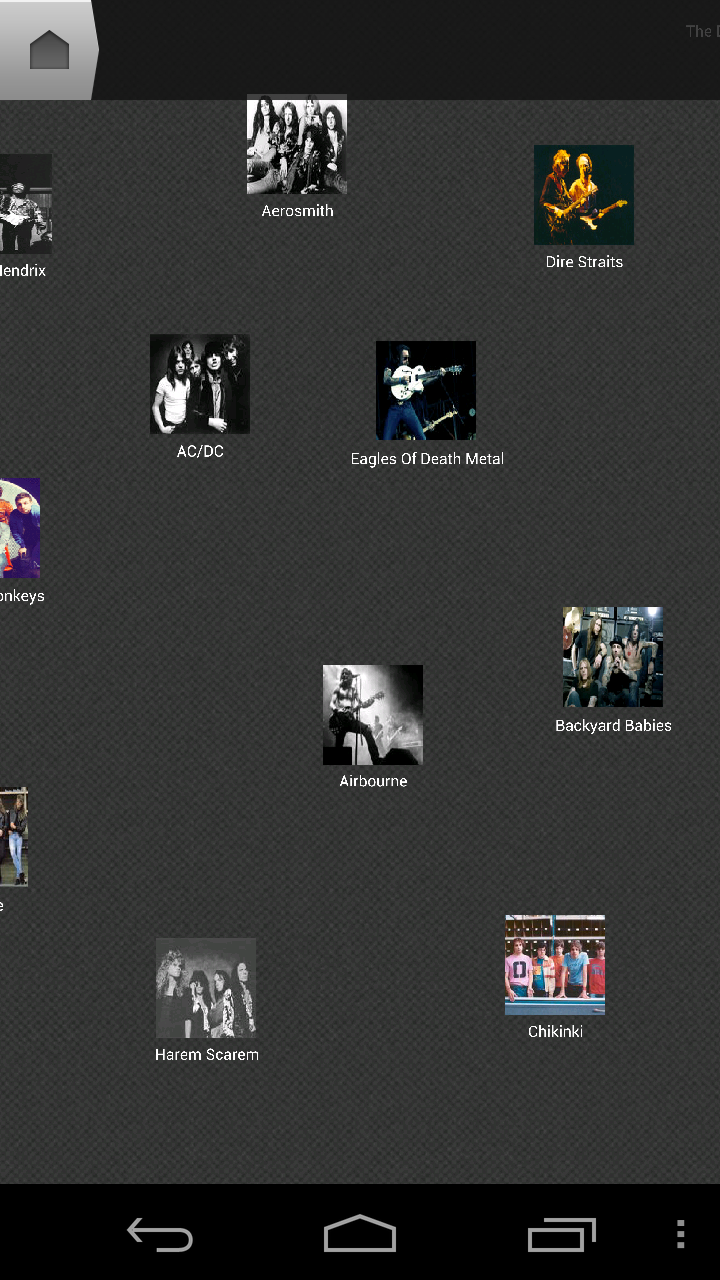
\includegraphics[width=0.4\textwidth]{figures/screen_mds_11_final_big_picture}
  \caption{Big picture of the graph state after the end of MDS computation}
\end{figure}

\section{Retrieval of Music Metadata}

\subsection{Querying of Music Metadata on the Device}

Android has a cursor-based query system for multimedia metadata (kept up-to-date transparently by the
operation system). Creation of a cursor for all artists on the device is performed by program code like this:

\begin{verbatim}
Cursor artistCursor = mContext.getContentResolver().query(
	MediaStore.Audio.Artists.EXTERNAL_CONTENT_URI,
    artistProjection, null, null, null);
\end{verbatim}

Since the returned metadata also contains a unique key for each multimedia file, metadata can be
persisted in a database (disconnected from the VM's memory) and later be reused without obstacles.
Metadata records themselves contain as much data as the user or the file-generating utility has defined
before the file was copied onto the device - clearly, files may not have any metadata available at all.

In the implementation of the App, such a cursor is traversed over all available music titles, and several entities are derived:

\begin{itemize}
	\item Artist,
	\item Album, and
	\item Track.
\end{itemize}

While these entities are created, the implementation checks whether they already exist, and skips creation accordingly. Retrieved data is then stored in the App's on-device database.

\subsection{Retrieval of Music Metadata from Websources}

Last.fm \cite{url:lastfm} and Echonest \cite{url:echonest} are the defacto standards for music metadata retrieval in the world wide web, 
at the time of writing of this paper. The author has chosen to use both of these services for retrieval 
of semantic metadata for the implementation. 

After the device's music titles and their metadata have been retrieved, their metadata has to be augmented or corrected with the normalized data from external sources - Last.fm and Echonest. To ensure a stable mapping from on-device to remote music metadata records, these are fetched up front. For every artist, album, and track the App has retrieved from the device, a match is searched for in web sources. Search for matches is performed by sending an ordinary search query to the web sources, and metadata records are returned as a result. Excerpts of the acquired records are then stored in the App's on-device database.

\section{Retrieval of Similarity Data}

Ideally, the retrieval of similarities between artists should provide an exhaustive list of similarities between any two artists. But, as a real-world implementation must make do with actuality, workarounds had to be found which provide approximations to artist similarities.
Echonest's artist similarity results contain no similarity metric, but only the implicit ranking of artists. Therefore, the author of this thesis decided \textbf{not to use Echonest's similarity metrics}.

Last.fm's artist similarity data is, in contrast to Echonest, augmented with accurate similarity measures in the range of $[0 .. 1]$. But, it is not possible to query Last.fm for a certain similarity relationship between two certain artists - instead, the top 100 similar artists for a certain artist can be retrieved. It's clear that this way, many artist-to-artist relations in a music collection will not receive a similarity measure. Instead, a dedicated algorithm has to approximate similarity values which were not provided by Last.fm.

As Last.fm provides similarity value lists per artist ("'subject"'), it can be assumed that every relation to an artist not on the list has a similarity value within the interval \emph{[0 .. x], x = lowest known similarity of "'subject"' to any other artist}. Not having any more details at hand than this fact, the expected value of such an unknown similarity value is $x / 2$ - the author of this thesis decided to use this value as an approximation.

\subsection{Similarity Approximation Algorithm}

In the following, the algorithm to interpolate similarity values (which is being used in the App's implementation) is described in simplified Java code:

\begin{verbatim}
for (artistOnDevice : allArtistsOnDevice) {
  similarArtists = LastFM.getSimilarArtists(artistOnDevice);
  for (innerArtistOnDevice : allArtistsOnDevice) {
    if (similarArtists.size() == 0)
      lowestMatch = 0;
    else
      lowestMatch = FLOAT_MAX;
    // Iterate through all found similarity matches:
    for (artistInLastFM : similarArtists) {
      // Find the lowest similarity match in the list:
      if (artistInLastFM.getSimilarityMatch() < lowestMatch)
        lowestMatch = artistInLastFM.getSimilarityMatch();
        // match is found, save a similarity object:
      if (matches(artistInLastFM, innerArtistOnDevice)) {
        artistSimilarity = new ArtistSimilarity(artistOnDevice, 
          innerArtistOnDevice, artistInLastFM.getSimilarityMatch());
        break;
      }
    }
	
    // No similar artists were returned at all:
    if (similarArtists.size() == 0)
      ArtistSimilarity artistSimilarity = new ArtistSimilarity(artistOnDevice, 
        innerArtistOnDevice, 0);    
    // Match was not found, save interpolated similarity object:
    else if (artistSimilarity == null)
      artistSimilarity = new ArtistSimilarity(artistOnDevice, 
      innerArtistOnDevice, lowestMatch / 2.0f);

    storeSimilarityIfNotExists(artistSimilarity);
  }
}	            
	
\end{verbatim}

\section{Implementation of Multidimensional Scaling}
\label{subch:implementation-mds}

The selected MDS algorithm has already been discussed broadly in section ~\ref{ch:computation}. Implementation of this algorithm required the creation of a number of helper and data classes, but on the whole, the implementation follows the pseudocode from section ~\ref{ch:computation} closely. To better illustrate step 3. from the mentioned pseudocode, the implementational part is included in the following as simplified Java code:

\begin{verbatim}
subject: the node to be positioned near any other node
initialSubset: the initial nodes subset of size sqrt(number of all nodes)
currentSubsetNodes: the nodes subset incrementally populated 
  by all remaining nodes not in the intial subset

nearestNode = getNearestNodeToSubject(subject, currentSubsetNodes);
distanceToNearestNode = distanceMatrix.getDistanceBetween(subject, nearestNode)
    * DISTANCE_CONSTANT;

// find out which quadrant (upper-l, lower-l, upper-r, lower-r) (where
// nearestNode is point zero) is suited best for subject:
upperRightQuadrant = getPointInQuadrant(1, 1, distanceToNearestNode, nearestNode);
lowerRightQuadrant = getPointInQuadrant(1, -1, distanceToNearestNode, nearestNode);
upperLeftQuadrant = getPointInQuadrant(-1, 1, distanceToNearestNode, nearestNode);
lowerLeftQuadrant = getPointInQuadrant(-1, -1, distanceToNearestNode, nearestNode);

// Add up the forces on the four representational quadrant points, for
// comparison later on:
upperRightStress = 0, lowerRightStress = 0, upperLeftStress = 0, lowerLeftStress = 0;
for (currentSubsetNode : currentSubsetNodes) {
    upperRightStress += getStress(subject, upperRightQuadrant, currentSubsetNode);
    lowerRightStress += getStress(subject, lowerRightQuadrant, currentSubsetNode);
    upperLeftStress += getStress(subject, upperLeftQuadrant, currentSubsetNode);
    lowerLeftStress += getStress(subject, lowerLeftQuadrant, currentSubsetNode);
}

// Find the quadrant point with the minimal stress, and move the subject
// there:
minStress = Min(Min(upperLeftStress, upperRightStress),
    Min(lowerLeftStress, lowerRightStress));
if (upperRightStress == minStress)
    subject.setPosition(upperRightQuadrant);
else if (lowerRightStress == minStress)
    subject.setPosition(lowerRightQuadrant);
else if (upperLeftStress == minStress)
    subject.setPosition(upperLeftQuadrant);
else
    subject.setPosition(lowerLeftQuadrant);

for (int i = 1; i <= QUADRANT_REFINING_ITERATIONS; i++) {
    // Improve on the quadrant point position by selecting a subset of
    // the initial graph subset, and reposition the subject such that
    // the stress between them and the subject is lowered:
    sumOfForcesOnSubject = new VirtualVector(0, 0);
    for (initialSubsetNode : initialSubset)
        sumOfForcesOnSubject.addVector(forceBetweenNodes(subject, initialSubsetNode));
    displaceNode(subject, sumOfForcesOnSubject);
}

currentSubsetNodes.add(subject);
	
\end{verbatim}

\section{Implementation of Removal of Node Overlappings}
\label{subch:implementation-overlapping}

The algorithm used for the removal of node overlappings has been shown in section ~/ref{ch:visualization}. The actual implementation required some pragmatic changes, therefore the code is listed in the following in simplified Java:

\begin{verbatim}
allNodes: all artists within the graph
nodesWithoutOverlap: artists within the graph which do not overlap with other artists
iterationsCount: number of iterations allowed to find a new position for one artist
nodesSize: diagonal through an artist's depiction square 
  (i.e., sqrt(x^2 + x^2) | x = artist node width and height), the maximally needed displacement
  to separate two overlapped artist nodes.
	
for (subjectNode : allNodes) {
  // move subjectNode around to find an empty spot for it among nodesWithoutOverlap
  for (i = 0; i < iterationsCount; i++) {
    for (collisionCandidate : nodesWithoutOverlap) {
      nodeCentersDistance = subjectNode.getEuclideanDistanceTo(collisionCandidate);
      randomMargin = random();
      if (nodeCentersDistance < nodesSize + randomMargin) {
        subjectNodeDisplacementVector = collisionCandidate.getVectorTo(subjectNode);
        subjectNodeDisplacementVector.setLength(nodesSize - nodeCentersDistance + random()); 
        subjectNode.move(subjectNodeDisplacementVector);
      }
    }
  }
  nodesWithoutOverlap.add(subjectNode);
}
\end{verbatim}

The optimized algorithm has a predefined number of iterations, by the end of which a node should no longer overlap any other nodes. This number has to be chosen carefully - too high and the overall computation duration will increase linearly, too low and not all node overlappings will be removed.

\section{Visualization Details}

Apart from the previously described computational algorithms, the App features a number of components or behaviour not contained in the Android operating system. In the following, the most interesting features aiding the visualization of content will be described.

\subsection{Drawing with OpenGL}

Android provides App developers with the possibility to implement threedimensional viewports in OpenGL ES \cite{url:opengles}, which is a downsized version of ordinary OpenGL and meant for implementation in handheld devices. OpenGL is a specification which is used as a blueprint by operating systems vendors and GPU producers alike. An OpenGL context can be seen as a state-machine which is manipulated by external API calls.

In order to be able to employ OpenGL for graph rendering, the author of this thesis had to create a number of abstract metaclasses and find a way to resemble user interactions in the drawn 3D picture. As mentioned before, the objective was to draw pseudo-2D, such that all music objects are displayed as pictures, viewed from the top. Accordingly, the viewport has to move sideways when the user moves one finger over the touchscreen, and it has to change its distance to the graph objects when the user zooms.

\subsection{Touchscreen Handling}

With the advent of smartphones, strong conventions have been established by phone vendors which determine how users may interact with the smartphone. Touchscreen technology provides a more immediate way of interaction than previous systems, allowing users to seemingly interact with the very objects they want to manipulate (as opposed to moving views and cursors with hardware buttons).
There are three touchscreen gestures supported by the App's implementation:

\begin{itemize}
	\item \textbf{Panning/Scrolling} - The user taps the finger onto the screen surface, does not let 
	go, and pulls the finger across the surface. As long as the finger does not part from the surface, 
	the "'pan/scroll"' is active.
	\item \textbf{Zooming} - The user rests two fingers on the screen surface, and changes the distance
	between her finger tips. If the distance decreases, then the zoom factor will increase; and vice versa.
	Ideally, the touched points would always stay right under the user's finger tips, but in the built
	App prototype, this has not been achieved, because of the threedimensional nature of the OpenGL
	rendering process.
	\item \textbf{Tapping} - The user taps her finger onto the screen surface at a point on which the
	desired object is located, and lets go again immediately. The App then reacts to this interaction
	with an adequate response or action, depending on the current state of the user interface.
\end{itemize}

\subsection{Animations}

To make transitions between view states in the App smoother and easier to follow for users, animations have been implemented to do so. It has been shown in an empirical study that comprehension of changes can be improved by adding animations ~\cite{Schlienger:2007}.

\textbf{Whole-screen transition} - If the user chooses to display an artist's albums, the transition to the next Activity (fullscreen Android layout component) is implemented as a fade-over animation, meaning that the second screen is added as an overlay and its alpha channel is animated from 0 to 1. This way, the user is able to notice the change of context without being disturbed by untracable changes.

\textbf{Artist Node animation} - If the user selects an artist by tapping, the artist's image depiction is moved on the z-axis towards the virtual camera - appearing nearer to the viewport. This puts an emphasis on the selected artist and makes for a pleasing optical effect. As OpenGL is a high-level framework, animations like this have to be implemented by the developer - keeping track of animation start and projected end time, and determining the state for every newly drawn frame.

\textbf{Context-related graph area darkening} - If the user chooses to display an artist's related (similar) artists, the graph area darkens over all other currently displayed artists, to put an emphasis on the selected artist and its related artists. This effect is achieving by adding a rectangle between the emphasized artists and the others, which is at first transparent and then gains opacity through an animation.

\section{Structure of the App}

\subsection{About Android Apps}

Android is a mobile operating system developed by the Open Handset Alliance ~\cite{url:openhandsetalliance}, led by Google. Its architecture allows for 3rd party programs (called "'apps"') to easily be run and debugged on Android devices.
Android apps are run in the Dalvik VM which makes use of a register-based architecture, relying on a Linux kernel for low-level functionality ~\cite{dalvik}. The most wide-spread programming language for building Android apps is Java, but various other languages such as Scala or even scripting languages like Groovy or Lua can be used. Since mid 2009, developers can also write and integrate native C and C++ code by making use of the Native Development Kit (NDK).

From an app developer's perspective, the frameworks contained in Android dictate a user-centric application structure, made up of so-called Activities ~\cite{url:androidactivity}. Every Activity encapsulates a screen which is presented to the user. Activities are loosely coupled, allowing only serialized objects and primitive values to be passed between them.

User interface composition in Android is performed partly in the CPU (e.g., in Java code), and partly in the device's GPU (by using the OpenGL interface). Apps can also choose between these composition variants.

Android is a strictly touch-centric operating system, meaning that most user interactions are performed via the device's touch screen. Originally, Android devices were bound to provide hardware buttons, but starting with Android 4.0, those buttons are gradually replaced with software buttons (displayed on the touch screen).

\subsection{App Components}

Activities
Helper Classes

\section{Summary of this Section}